\chapter{Multi-task learning}
Multi-task learning is a generalization of Transfer Learning to training a single model where the goal is to optimize for multiple objectives. 
Training a multi-task model requires a set of distinct tasks to be posed as a multi-task learning problem.
It can have many benefits when applied correctly, such as making the models more general by regularization and reducing computational requirements.
On the other hand, if multi-task learning is applied to problems that don't train well in a multi-task setting, the resulting models can be significantly worse than the single-task counterparts.
Here we look at examples of multi-task learning in computer vision.
Especially recently, with the introduction of transformers like BERT \citep{bert}, multi-task learning and transfer learning have gained popularity within natural language processing, but to restrict our scope, we only consider how to apply multi-task learning in computer vision. 

\section{Definition}
Multi-task learning is quite similar to transfer learning. 
However, the main difference lies in the fact that the goal is to generalize to solve and improve performance in all tasks using some shared representation. 
In contrast, transfer learning aims to optimize a single new task, ignoring the performance on the original task entirely. 
Often in multi-task learning, the shared layers are initialized using some ImageNet model and transfer learning as the ImageNet backbone is an architectural feature shared in many models.

The formal definition for multi-task learning follows the definition given in \citep{surveyOnMultiTask}. 
A learning problem consists of ${m}$ related learning tasks ${\{T_i\}_{i=1}^m}$ that are trained together. 
Each task has a dataset ${D_i}$ with ${n_i}$ pairs ${\{x_{j}^{i}, y_{j}^{i}\}_{j=1}^{n_i}}$, where ${x_{j}^{i}}$ refers to the input of task ${T_i}$ and ${y_{j}^{i}}$ is the label corresponding to the input vector.
Let ${X^i}$ = (${x_{1}^{i}, ... , x_{n_i}^{i})}$ be the input matrix for task ${T_i}$.
In a multi-task setting there can be ${x}$ such that ${x \in X^i}$ and ${x \in X^j}$ or ${X^i = X^j}$ for some ${i \ne j}$, meaning that a single image has multiple labels or an entire data set has labels for multiple tasks.

To train the network, each task ${T_i}$ needs to have its loss function defined.
A commonly used way to get the total loss of the input is by using the weighted loss functions for all tasks, resulting in a formula \[L_{total} = \sum_i{w_i L_i}\] \noindent, where ${L_i}$ is the loss function for task ${T_i}$ and ${w_i}$, is the weight that specifies the sensitivity of the task \citep{usingUncertaintyToWeighLosses}. 
The sensitivity multiplies the loss of the task.
Multiplying the loss has the effect of making the error on the task with higher sensitivity to have a larger impact on the adjustment of weights.
So the sensitivity should be used to either pick tasks that are important or to normalize the losses if they are very different.
There can be significant differences in the scale of the losses if different tasks use different loss functions.
The sensitivity of the tasks is an essential parameter to get right as choosing a too high parameter for some task might lead to a solution that is optimal for only the most sensitive task, starving the others \citep{whichTasks}.

Once the loss function is specified, the actual training is quite similar to training a single-task model.
The one new thing to consider in a multi-task setting is the sampling ratio of the different tasks as some tasks can be easier to learn or contain significantly more or less data compared to other tasks.
Like in regular training, the models are trained one batch at a time. 
In a multi-task setting, we have datasets for each of the tasks from which we can pick at a time.
Now, we can define an epoch e in the training process as the total number of batches from all tasks. 
The epoch can be formalized as \[ e = \sum_i{ \dfrac{|X_i| \alpha_i}{B_i}}\] \noindent batches over $i$ tasks, where $|X_i|$ is the training set size, $B_i$ is the batch size, and $\alpha_i$ is the scaling factor for each task, telling how important the specific task is for the learning process.
The sampling ratio is one of the new parameters that is required when doing multi-task learning on multiple datasets.
When training models, some value has to be picked for the sampling ratios, and picking wrong values leads to worse models.
Precisely what is a good sampling ratio is complicated to tell beforehand, and generally, the chosen values need to be evaluated by experimentation.
Iterating through all batches can be done in a round-robin fashion, by going through all batches of each data set at a time or randomly sampling the sets with probabilities respective to their magnitude and scaling factor.

\section{Latent image representations}
For a multi-task model, the optimal situation is such, where all classifiers would use a single shared latent representation of the image to predict all attributes.
This representation is an image embedding, that would capture all valuable information of the image for our tasks.
The embedding could be the vector represented by the final layer of an ImageNet classifier flattened to some n-dimensional vector that then solves all the tasks instead of just a single task.
\begin{figure}[h!] 
\centering 
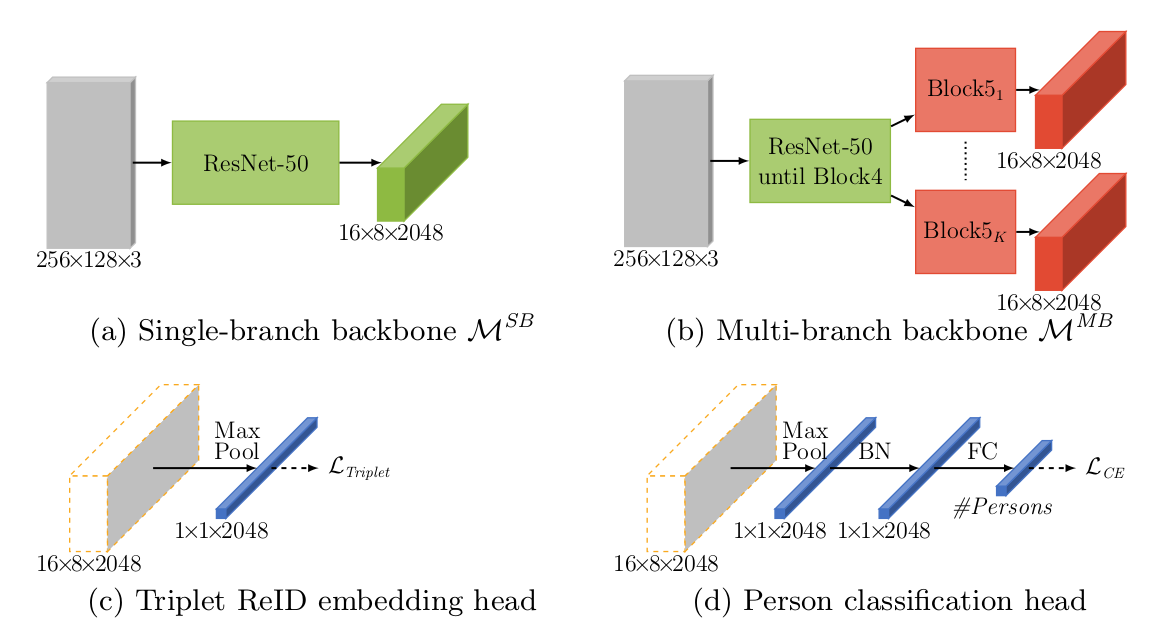
\includegraphics[width=0.8\textwidth]{imgs/sharedBackbone.png}
\caption{Example of partly and completely shared backbones. Figure from \citep{visualPerson}.\label{fig:params}}
\end{figure}
However, such a universal image representation can be challenging or impossible to learn, and instead, only a part of the network is shared between the tasks.
Here, this shared structure is called the backbone of the multi-task classifier.
Often the backbone is in the form of some ImageNet classifier architecture, and it can be the entire classifier or some layers up to some arbitrary limit.
As the amount of layers shared is picked for each task separately, some tasks can share the entire classifier as a backbone, and others might only share some amount of layer that produces desirable results.

Besides just deciding the network branching, each task requires an independent head that outputs prediction for that task.
These task heads are similar to those used in transfer learning, where only a single task is solved using the ImageNet backbone.
Especially in a multi-task setting, these heads can be more than just a single linear layer calculating the softmax over all classes.
A single head can contain any combination of several linear layers, dropout layers, batch normalization layers, convolutional layers, or it could be a Recurrent Neural Network creating a caption for the image embedding, depending on the task at hand.
In Figure 4.1, we can see an example of the flexibility of the sharing as the model can use a completely shared backbone or a branching backbone, which has a unique head for each task, solving the person re-identification and classification tasks.

\section{Benefits}
Depending on how and where multi-task learning is applied, it can provide a multitude of benefits to the model.
Many of these benefits stem from the fact that the model gets to see more data, and the various tasks can make it easier to find useful features.
Different kinds of data sets have different kinds of noise, learning multiple tasks makes it easier to distinguish which features are beneficial and detrimental some features may be difficult to learn on a dataset but can be useful and borrowed from another and learning multiple tasks forces the model to not overfit on one of them \citep{ruderOverview}.

These benefits come up when the tasks are compatible and allow the model to learn more general features, generally leading to better performance on the distinct tasks. 
When the needed features between tasks are conflicting, the model performance tends to go down \citep{uberNet}.
The problem of deciding what to share is not easy to solve.

The benefits of multi-task learning come up, especially when dealing with limited amounts of data, in which case, particularly finding the features that matter without overfitting can be complicated. 
For example \citep{biologicalMultitask} found that multi-task learning could improve gene expression pattern classifiers when trained in a multi-task setting. 
The multi-task classifier was significantly better than the one only using transfer learning, showing that the features learned were more general.

Another significant boon of multi-task models, especially in embedded domains, is the reduction in model size and inference time. 
As many classifiers are dependent on an embedding of an image to produce results, using a shared embedding of an image for multiple tasks means that the model requires only a single partly or completely shared backbone. 
For example \citep{multiPoseNet} uses a shared backbone to detect people in an image and to detect keypoints on their body and then finally to do a semantic segmentation of the image while also improving performance on most of the tasks.

Finally, a model using multi-task learning can take advantage of the different losses to produce a more optimal loss weighing strategy compared to constant weighting. 
Picking the weights in the total loss function is very important as with invalid weights, the optimization can be difficult or even impossible \citep{lossWeighting}. 
The weights become even more critical if the losses for various tasks are different, for example, one task might use mean squared error as a loss function and another cross-entropy, and the resulting loss values might differ by orders of magnitude.
The total loss function can be modified by adding an uncertainty weighting to each of the tasks by considering the uncertainty of the prediction \citep{usingUncertaintyToWeighLosses}. 
Depending on the task, the benefit compared to an unweighted loss can be significant \citep{usingUncertaintyToWeighLosses} or, in some cases, only small \citep{lossWeighting}.

\section{Hard parameter sharing}
A hard parameter sharing setting is one where the same convolutional weights in the intermediate layers solve multiple tasks, like in Figure 4.1.
Hard parameter sharing is the primary way of reducing total model size and inference time when solving multiple tasks simultaneously.
While sharing the weights can provide many benefits to the end model, as seen in the previous chapter, it comes at the cost of an increased number of tunable parameters when training the models. 
As we have previously seen, multi-task models introduce new constant factors to the training process beyond the normal hyperparameters for learning rate, dropout rate, and others.
These include the hyperparameters for weighing the loss functions and determining the task sampling ratios, but also the expensive to evaluate architectural decision of which tasks should share representations and how much should be shared.

\begin{figure}[h!] 
\centering 
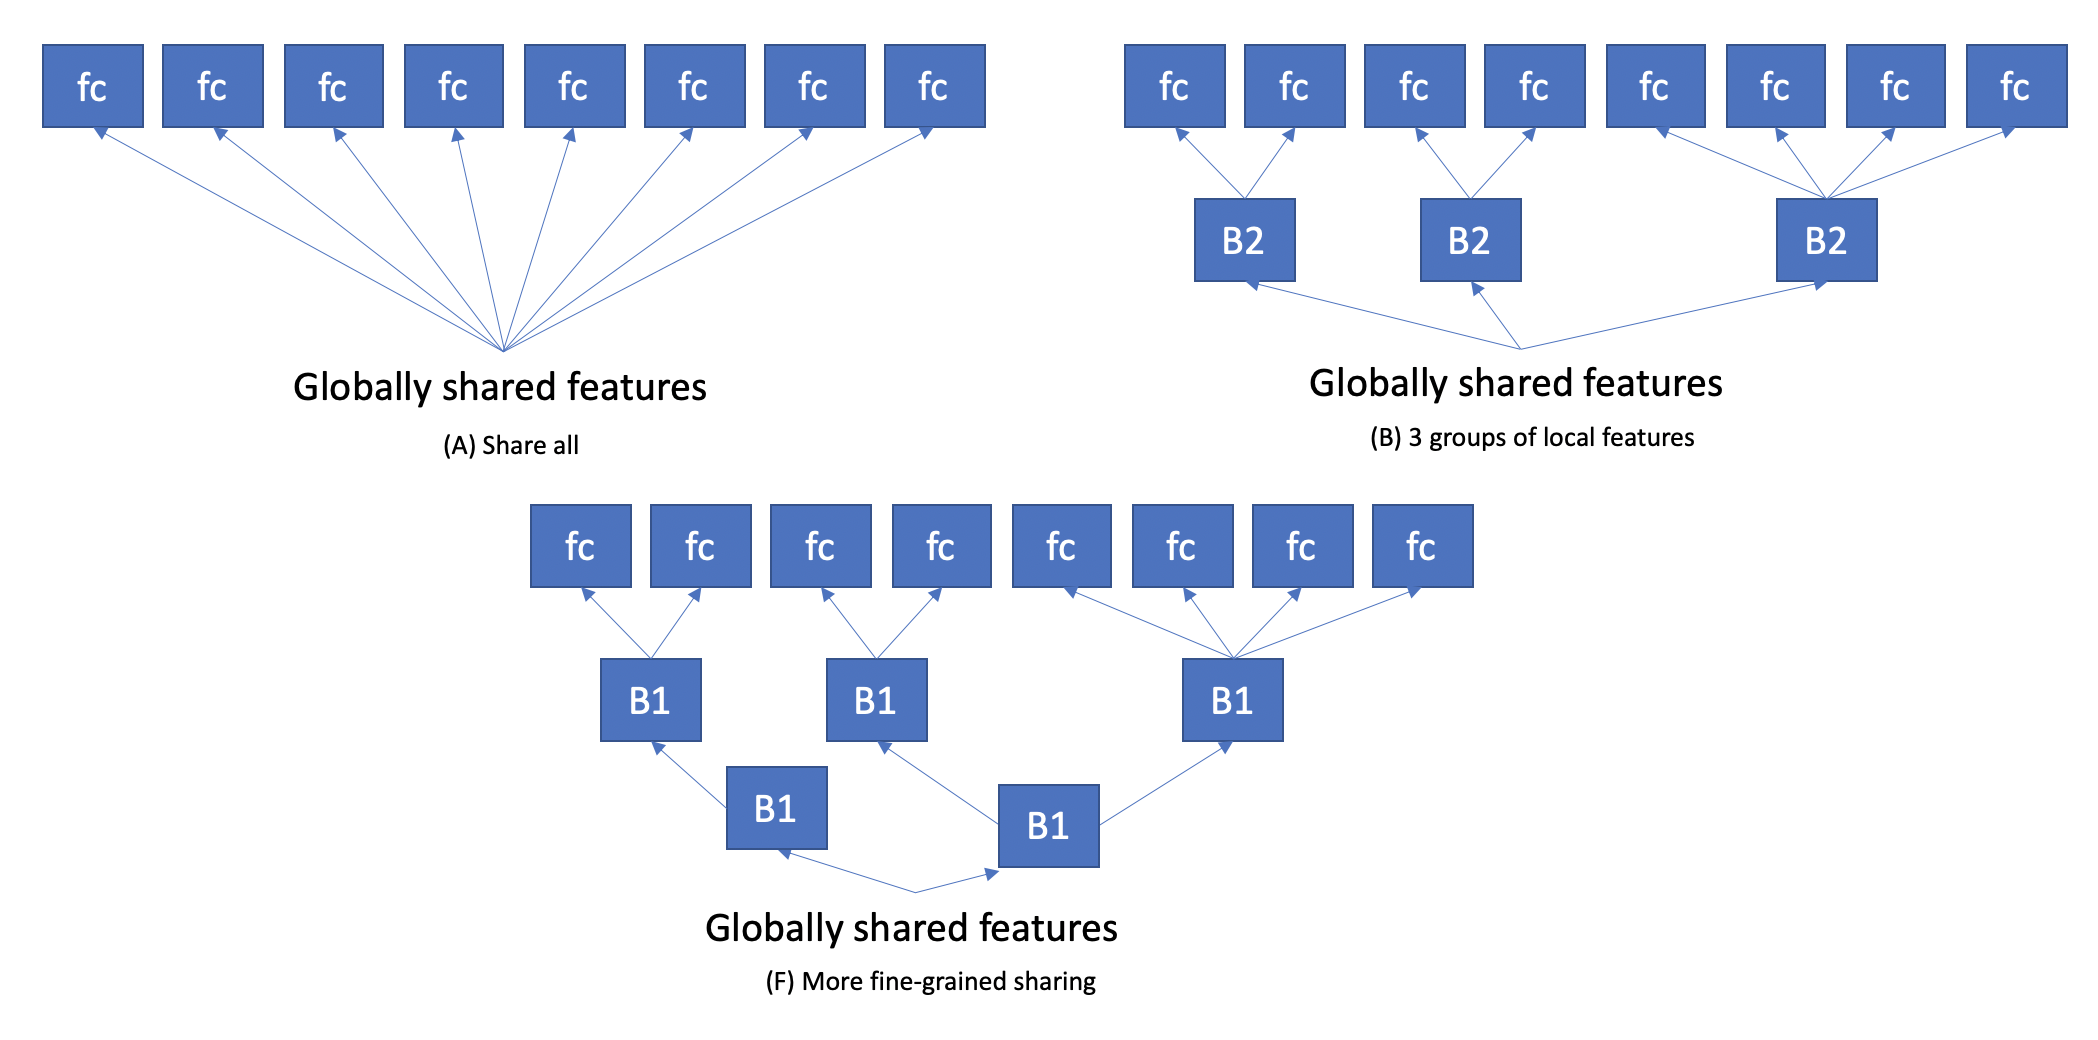
\includegraphics[width=1\textwidth]{imgs/multipleShares.png}
\caption{Some ways of sharing features between tasks. Here the global features are from resnet. The fc blocks are fully-connected heads. B1 is one ResNet block and B2 is two ResNet blocks. Out of these model F was the best. Figure adapted from \citep{healthyDrink}.\label{fig:params}}
\end{figure}

In Figure 4.2, there are multiple ways of configuring a multi-task network in terms of what to share.
The results for the different configurations were quite varied. 
However, even the worst multi-task Model A did better on every task when compared to the single-task models, and accuracy improvement from the single-task case to the best multi-task Model F was roughly 20\% \citep{healthyDrink}.
These results are quite validating for the presumed benefits of multi-task models.
Since these results show that it is possible to share the majority of the network parameters and, at the same time, increase the performance, even with the most greedy share-all model.
Though, at the same time, it shows that multiple compute-expensive experiments have to done to find the most optimal sharing structure for the backbone network.

In the experiments done by \citep{healthyDrink}, they utilized auxiliary training to great effect.
They had two original features of interest that were sugar and alcohol level in the drinks.
Other features were added as auxiliary training features to improve the performance on the two original features \citep{healthyDrink}.
This auxiliary training can also be done by, for example, using ImageNet to keep the original classifier accurate on ImageNet while training on the new data set like in \citep{biologicalMultitask}; this way, the model won't be able to overfit on the new data so easily.
In the drink classification experiment, the auxiliary tasks were picked in a way that they might help in finding the correct features to solve the actual tasks \citep{healthyDrink}.
Adding auxiliary tasks is an interesting way of forcing features into the model that the developer thinks could be useful for the model to find, in that sense, they are hand-crafted features that get augmented in the model.
In practice, this means that if we are training a model e.g., to predict the steering angle given an image, we might want to add an auxiliary task that predicts the lane markers to make it easier to learn these features as they should be a significant feature for producing correct outputs.

A similar multi-task model in \citep{visualPerson}, also partly visualized in Figure 4.1, solves 6 different tasks in a single model.
The tasks in that model are very different from one another, including person re-identification, pose estimation, and image segmentation.
The interesting result in their search for related tasks is that while a pair of tasks don't work well together, they can work well when combined with other tasks.
For example, they found that just pairing the pose estimation head with other tasks significantly reduces its accuracy, but when all tasks use the single shared backbone, it does just as well as if trained in a single-task setting.
These results show that very different tasks can combine to a single model to provide a very significant reduction in model size while producing about as good or better accuracies.

\section{Soft parameter sharing}

\begin{figure}[h!] 
\centering 
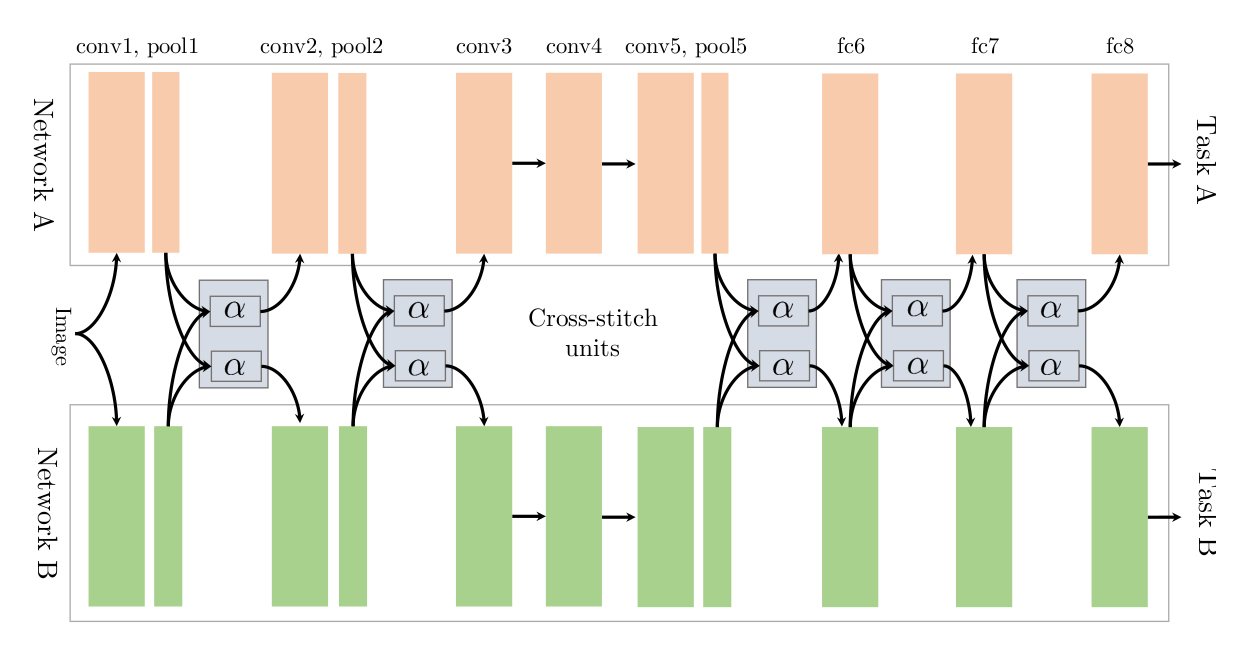
\includegraphics[width=0.8\textwidth]{imgs/stitch.png}
\caption{Cross-stitch architecture. Figure from \citep{crossStitch}.\label{fig:params}}
\end{figure}

Soft parameter sharing is quite similar to learning each task on its own since each task has separate weights. 
Soft parameter sharing happens by picking some layers, where some metrics constrain the parameters to be similar, like ${l_2}$ distance \citep{ruderOverview}. 

The sharing functionality can be more complicated than just basic regularization. 
For example, the Cross-stitch units \citep{crossStitch} are a particular type of soft sharing, where the stitch units combine tasks A and B using a linear combination of the activations, visualized in Figure 4.3. 
The benefit here is that the user does not need to specify how much should be shared between the tasks, but it is instead learned in the cross-stitch unit. 
If nothing needs to be shared, then the network can learn to assign the weight for the other task to zero.

This kind of sharing does not scale very well as the number of tasks increases since calculating the relation between various tasks is quadratic. 
Since the joining logic requires extra parameters, it means there is even more to learn than just learning all the tasks separately. 
As soft sharing does not provide many of the benefits that are gained by hard sharing the parameters, it is not as popular.
However, it is useful in adding some extra information between the tasks to gain extra performance by utilizing the latent representations between them in various ways.
Also, in the basic case of using a soft parameter share to constraint, the layers can improve the generalizability of the model.

\section{Attention augmented Multi-task learning}
In a multi-task setting, the model ends up having a representation of the image from each task's point of view, and it is possible to use attention \citep{attention} to augment the predictions.
Especially in the case where the tasks are heavily correlated, this can be quite useful.
For example, when doing weather recognition, it would make sense that some of the features are correlated, and this correlation can be used by adding an attention layer between the different tasks, like in \citep{cnn-rnn}.
The Multi-Task Attention Network (MTAN) \citep{multiTaskAttention} is an example of a more advanced application of attention in multi-task models.
In the MTAN, each task gets its own attention module, and they are used to determine correlations of the tasks at specific layers of the network using the attention operations.
It is similar to cross-stitching networks in that each task has to learn its attention module features. 
However, there is only a single backbone for the shared features, and the attention modules are responsible for producing the task level outputs.
The number of parameters is still significantly reduced as the task specific-parts are not complete ImageNet classifiers, resulting in a significantly more efficient and accurate classifier for image segmentation.

\section{What and when to share}
What makes or breaks a multi-task model is the decision on what should be shared, but determining what and how much should be shared is exponentially more expensive as the number of tasks grows.
Currently, there is no definitive way of theoretically evaluating which tasks should have a shared representation and just how much can be shared.
As experimentation is expensive, a good starting point is to try to find similar tasks that should do well together. 
However, there is no guarantee that even all the tasks within a single family of problems are beneficial for joint training, so some experimentation has to be done. 
The desired result in a multi-task setting would be to share all the parameters between all the tasks, but as can be seen in \citep{uberNet}, that approach often significantly reduces performance.
If sharing an entire network does not produce good results, it can be a good idea only to share some part of it as the lower level features tend to be more general \citep{transferringMidLevelRepresentations}. 
By sharing only a part of the network, it may be possible to strike the right balance between performance and model complexity.

\begin{figure}[h!] 
\centering 
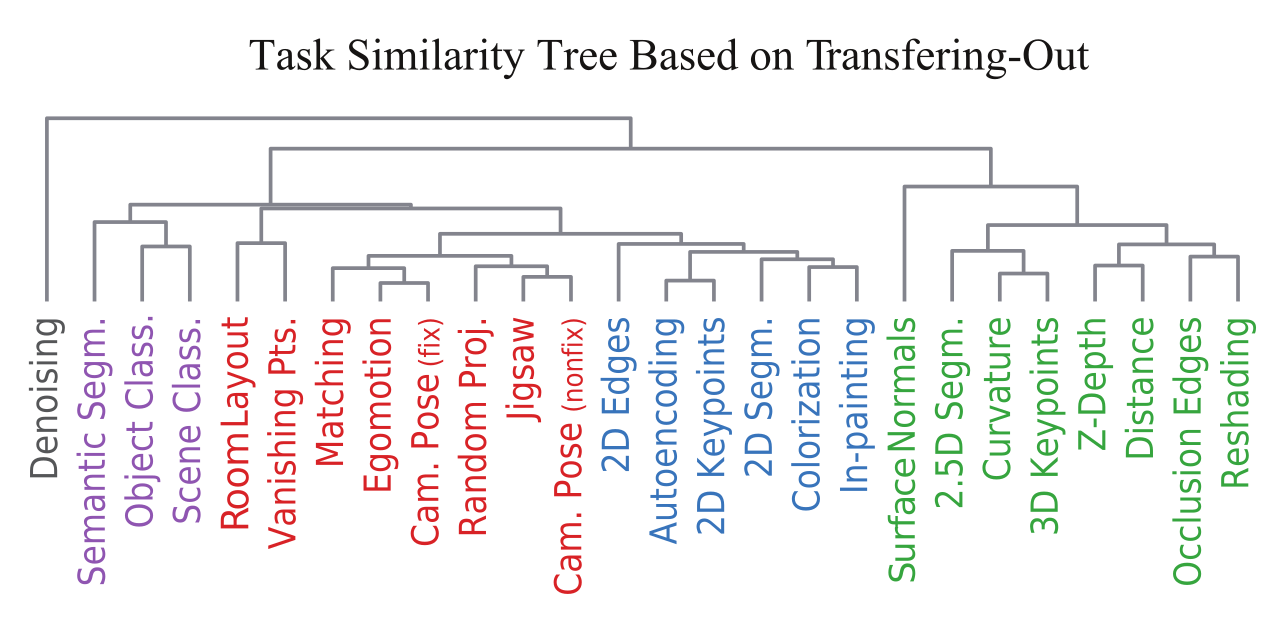
\includegraphics[width=0.8\textwidth]{imgs/taskonomy.png}
\caption{The taskonomy task similarity tree. Figure from \citep{taskonomy}.\label{fig:params}}
\end{figure}

An attempt to create a taxonomy of related tasks called Taskonomy to find out what tasks are beneficial for transfer learning exists in \citep{taskonomy}. 
The Taskonomy experiments pre-trained networks on tasks and then evaluated whether the features would transfer well to other tasks to end up with a hierarchical categorization of related tasks, shown in Figure 4.4. 
Still, the authors noted that, depending on model architecture and data set, the results could be different.

It would make sense that the results of the Taskonomy would be easily transferable to the multi-task setting. 
When evaluating the multi-task vs. transfer affinity, it turns out that they are negatively correlated, at least in the case of the five tasks that were the focus of the experiments in \citep{whichTasks}. 
Based on this observation, it can be beneficial to train some non-related tasks together. 
The authors suggest that the different tasks act as a good form of regularization as the models need to generalize to multiple types of inputs. 
It could also be that some of the learned features work very well for the other task, but can't be easily learned with the dataset of the other task and vice versa.
These results are aligned with the empirical results that we saw when we looked at the compatibility of classifiers using hard weight sharing.
Currently, it seems not to be possible to determine the compatibility of different tasks purely on a theoretical grounding.
Instead, experiments need to be run, and the results of pairs of tasks do not always generalize to a set of all other tasks when using shared representations in models \citep{visualPerson}.
